\chapter{Migration process}

This chapter describes the process of migrating a web application to serverless architecture. The goal of the migration is to explore the feasibility of the catalogued patterns by applying them on common problems in the domain of web application development. In cases where the patterns prove insufficient or unsuitable to the problem in hand, modifications or new patterns are proposed. As well as exploring the patterns we're also seeing how the distinct serverless features drive application design and trying to gain deeper understanding of the advantages and shortcomings of the paradigm.

The migrated application is a tool for managing image assets, adapted from a real-world work assignment. Similarly to SaaS offerings such as Cloudinary, the application takes user-uploaded images, does various forms of processing and then serves the processed images publicly to be consumed by other applications. In our case the processing needs are threefold: rendering a thumbnail, rendering a low quality image placeholder (LQIP), and automatic labelling using an external image analysis API. In addition the application does CAPTCHA-based authentication to protect the image upload endpoint from abuse.

We can thus roughly divide the application into three parts: image hosting, image processing and authentication.

Figure \ref{fig:imageManager} presents the pre-migration serverful architecture. In this implementation all image processing logic as well as the various service clients are contained inside a single server application that is then hosted on a VM. \ref{fig:serverlessImageManager} presents the migrated serverless architecture, where the same functionality is split into separate serverless functions and tied together in an event-driven flow. In both figures rectangular boxes represent the parts that are implemented by hand, whereas the rest are external services.

TODO serverful app already uses cloud storage and analysis API

Building both deployment artifacts from the same code base

\begin{figure}[h]
  \centering
  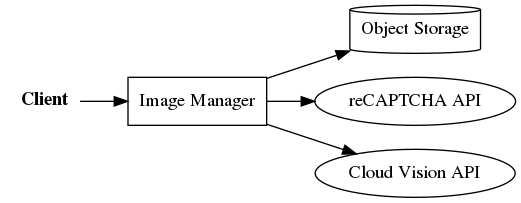
\includegraphics[width=0.65\textwidth]{image-manager.png}
  \caption{Serverful Image Manager}
  \label{fig:imageManager}
\end{figure}

\begin{figure}[h]
  \centering
  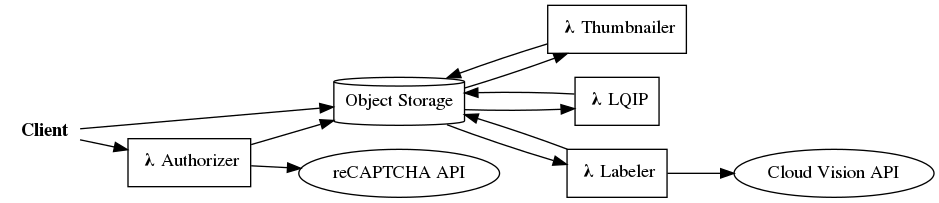
\includegraphics[width=\textwidth]{image-manager-serverless.png}
  \caption{Serverless Image Manager}
  \label{fig:serverlessImageManager}
\end{figure}

\section{New patterns} \label{sec:newPatterns}

Here are some patterns to address problems I came across while sketching out the above serverless implementation:

\subsection{Fetcher} \label{subsec:Fetcher}

\textbf{Problem:} Scaling an IO-bound operation out to parallel function instances is inefficient since the instances compete of the same IO resources.

\textbf{Solution:} Use local threading inside a single function instance to efficiently scale out operations like network requests.

E.g. three parallel functions each making a network request, or three parallel functions invoked by cloud storage upload that start execution by downloading the image: is it more efficient to have one function download the image and then invoke/pass the image as argument to three processing functions?

\subsection{Asynchronous Response} \label{subsec:AsyncResponse}

\textbf{Problem:} The client doesn't get any feedback from the asynchronous tasks it triggers.

\textbf{Solution:} Use a pub/sub channel to send a message to the client at the end of the task.

\subsection{Task Manager} \label{subsec:taskManager}

\textbf{Problem:} The client, after triggering an asynchronous task, has no way of tracking task progress or cancelling it.

\textbf{Solution:} Make each function instance subscribe to a pub/sub channel in the beginning of its execution in order to listen to client commands.

\subsection{Throttled Recursion} \label{subsec:throttledRecursion}

\textbf{Problem:} Recursive serverless functions can overwhelm downstream resources by scaling out quickly or result in an infinite loop.

\textbf{Solution:} Pass recursive invocations through a message queue in order to control recursion speed.
